\documentclass[12pt,handout]{beamer}

%\documentclass{beamer}
\usetheme{Boadilla}
\useoutertheme{split}
\usepackage{fancyvrb}
\usepackage{tikz}
\usepackage{svg}
\usetikzlibrary{shapes, calc, shapes, arrows, datavisualization}

\usepackage{amsmath,amssymb}

\definecolor{myblue}{RGB}{80,80,160}
\definecolor{mygreen}{RGB}{80,160,80}


\title{Gettting Started with Gurobi}
\author{Abr\`emod Training}
\titlegraphic{
\includegraphics[scale=0.1]{abremodlogo.png}}


\begin{document}

\begin{frame}
\titlepage
\end{frame}

\begin{frame}
\frametitle{Overview}
\begin{itemize}
\item Linear Programming (LP)
\item Solving LPs with Gurobi
    \begin{itemize}
    \item Interactive Shell (Python)
    \item .NET Interface
    \end{itemize}
\item LP Modeling Techniques
\item Multi-Objective Optimization
\item Integer Programming
\item Performance Tuning
\item Column Generation
\item Convex Quadratic Programming
\item Stochastic Programming
\end{itemize}
\end{frame}

\begin{frame}
  \frametitle{Abr\'emod}
Abr\'emod specializes in implementing math programming models to solve business problems.
Including business analysis, modeling, and implementation.
\begin{itemize}
\item Revenue Management
\item Assignment/Scheduling Problems
\item Network Optimization
\end{itemize}
\end{frame}

\begin{frame}
\frametitle{What is a Mathematical Program?}
\begin{itemize}
\item Decision Variables (what you control)
\item Constraints (rules you must follow)
\item Objective Function (what you want to minimize/maximize)
\end{itemize}
\end{frame}

\begin{frame}
\frametitle{What is a Mathematical Program?}
\begin{block}<+->{Definition}
%\begin{align*}
\begin{eqnarray}
\mbox{minimize/maximize:} && f(x_1, x_2, \ldots, x_n) \nonumber \\
\mbox{subject to:} && g_i(x_1, x_2, \ldots, x_n)
\begin{Bmatrix}   \le \\
                   \ge \\
                   =
\end{Bmatrix}
b_i, \;\; i = 1, \ldots, m \nonumber \\
&& x_j \ge 0,\;\;j = 1, \ldots, n \nonumber
\end{eqnarray}
%\end{align*}
\end{block}
\end{frame}

\begin{frame}
\frametitle{Math Programming Terminology}
\begin{itemize}
\item $x_j$ are the {\em decision variables}.
\item $g_i(x_1, x_2, \ldots, x_n) \begin{Bmatrix}   \le \\
                    \ge \\
                    =
\end{Bmatrix} b_i$ are {\em structural constraints}.
\item $x_j \ge 0$ are {\em nonnegativity constraints}.
\item $f(x_1, \ldots, x_n)$ is the {\em objective function}.
\item A {\em feasible solution}, $\hat{x} = (\hat{x}_1, \ldots, \hat{x}_n)$ satisfies all constraints.
\item The {\em feasible region} is the set of all feasible solutions.
\item The objective function ranks the feasible solutions.
\item The optimal solution $x^*$ satisfies $f(x^*) \le f(\hat{x})$ for all feasible $\hat{x}$.
\begin{itemize}
\item $x^*$ is feasible itself.
\end{itemize}
\end{itemize}
\end{frame}

\begin{frame}
\frametitle{The Linear Program}
\begin{eqnarray}
z^* = \mbox{minimize:} && c_1 x_1 + c_2 x_2 + \cdots + c_n x_n \nonumber \\
\mbox{subject to:} &&a_{i1} x_1 + a_{i2} x_2 + \cdots + a_{in} x_n
\begin{Bmatrix}   \le \\
                   \ge \\
                    =
\end{Bmatrix}
b_i,\;\;i = 1,\ldots,m \nonumber \\
&&x_1, x_2, \ldots, x_n \ge 0 \nonumber
\end{eqnarray}
In standard matrix form:
\begin{eqnarray}
z^* = \min_{x} && c^T x \nonumber \\
\mbox{s.t.} && Ax = b \nonumber \\
&& x \ge 0 \nonumber
\end{eqnarray}
\end{frame}

\begin{frame}
\frametitle{The Linear Program}
\begin{eqnarray}
z^* = \mbox{minimize:} && c_1 x_1 + c_2 x_2 + \cdots + c_n x_n \nonumber \\
\mbox{subject to:} &&a_{i1} x_1 + a_{i2} x_2 + \cdots + a_{in} x_n
\begin{Bmatrix}   \le \\
                   \ge \\
                    =
\end{Bmatrix}
b_i,\;\;i = 1,\ldots,m \nonumber \\
&&x_1, x_2, \ldots, x_n \ge 0 \nonumber
\end{eqnarray}
\begin{itemize}
\item $a_{ij}$, $c_j$, and $b_i$ are data.
\item Find $x^*$ satisfying $c_1 x_1^* + \cdots + c_n x_n^* \le c_1 \hat{x}_1 + \cdots + c_n \hat{x}_n$ for all feasible $\hat{x}$.
\item A linear program (LP) is a special type of math program with:
    \begin{itemize}
    \item $f(x_1,\ldots,x_n) = c_1 x_1 + \cdots + c_n x_n$
    \item $g_i(x_1,\ldots,x_n) = a_{i1} x_1 + \cdots + a_{in} x_n,\;\;i = 1,\ldots,m$
    \end{itemize}
\end{itemize}
\end{frame}

\begin{frame}
\frametitle{Linear Programming Axioms}
\begin{eqnarray}
z^* = \min / \max && c_1 x_1 + c_2 x_2 + \cdots + c_n x_n \nonumber \\
\mbox{subject to:} &&a_{i1} x_1 + a_{i2} x_2 + \cdots + a_{in} x_n
\begin{Bmatrix}   \le \\
                   \ge \\
                    =
\end{Bmatrix}
b_i,\;\;i = 1,\ldots,m \nonumber \\
&&x_1, x_2, \ldots, x_n \ge 0 \nonumber
\end{eqnarray}
\begin{itemize}
\item Additivity
\item Proportionality
\item Divisibility
\item Certainty
\end{itemize}
\end{frame}

\begin{frame}
\frametitle{The Diet Problem}
There are 5 types of food and two nutrient requirements that we must satisfy at minimum cost.
\begin{center}
Units of nutrients and cost per ounce
\begin{tabular} {c | c | c | c}
Food type & Iron & Calcium & Cost \\
\hline
1 & 2 & 0 & 20 \\
2 & 0 & 1 & 10 \\
3 & 3 & 2 & 31 \\
4 & 1 & 2 & 11 \\
5 & 2 & 1 & 12 \\
\end{tabular}
\end{center}
Nutrient requirements: 21 units of iron and 12 units of calcium
\end{frame}

\begin{frame}
\frametitle{Diet Problem Formulation}
\begin{columns}[t]
\begin{column}{4cm}
\begin{center}
\begin{tabular} {c | c | c | c}
Food & \#1 & \#2 & Cost \\
\hline
1 & 2 & 0 & 20 \\
2 & 0 & 1 & 10 \\
3 & 3 & 2 & 31 \\
4 & 1 & 2 & 11 \\
5 & 2 & 1 & 12 \\
\end{tabular}
\end{center}
Nutrient requirements: \\ Iron: 21, Calcium: 12
\end{column}
\begin{column}{7cm}
\begin{itemize}
\item Decision Variables
    \begin{itemize}
    \item $x_j = $ \# of ounces of food type $j = 1, 2, \ldots, 5$
    \end{itemize}
\item Objective Function
    \begin{itemize}
    \item min $z = 20 x_1 + 10 x_2 + 31 x_3 + 11 x_4 + 12 x_5$
    \end{itemize}
\item Structural Constraints
    \begin{itemize}
    \item $2 x_1 + 0 x_2 + 3 x_3 + 1 x_4 + 2 x_5 \ge 21$
    \item $0 x_1 + 1 x_2 + 2 x_3 + 2 x_4 + 1 x_5 \ge 12$
    \end{itemize}
\item Nonnegativity constraints
    \begin{itemize}
    \item $x_j \ge 0, j = 1, 2, \ldots, 5$
    \end{itemize}
\end{itemize}
\end{column}
\end{columns}
\end{frame}


\begin{frame}
\frametitle{Solving with the Gurobi Interactive Shell}
\begin{itemize}
\item Objects and Methods you will need (.NET equivalent)
    \begin{itemize}
    \item Model (GRBModel)
        \begin{itemize}
        \item addVar(lb, ub, obj, vtype, name)
        \item addConstr(constr, name)
        \item update()
        \item optimize()
        \end{itemize}
    \item Var (GRBVar)
        \begin{itemize}
        \item X
        \item RC
        \end{itemize}
    \item Constr (GRBConstr)
        \begin{itemize}
        \item Pi
        \item Slack
        \end{itemize}
    \end{itemize}
\end{itemize}
\end{frame}

\begin{frame}
\frametitle{Querying the Solution}
\begin{itemize}
\item Model.write()
    \begin{itemize}
    \item m.write('diet.lp') outputs the model in human-readable form
    \item m.write('diet.mps') outputs a full-precision copy of the model
    \item m.write('diet.sol') outputs the solution
    \end{itemize}
\item Model object attributes
    \begin{itemize}
    \item m.NumConstrs
    \item m.NumVars
    \item m.Status (was the solver able to find an optimal solution?)
    \item m.ObjVal (optimal objective value)
    \end{itemize}
\end{itemize}
\end{frame}

\begin{frame}
\frametitle{Querying the Solution}
\begin{itemize}
\item Var object attributes
    \begin{itemize}
    \item x1.X - optimal value
    \item x1.RC - reduced cost, change in objective/change in variable bound
    \end{itemize}
\item Constr object attributes
    \begin{itemize}
    \item iron_constraint.Pi - shadow price, change in objective/change in RHS
    \item iron_constraint.Slack - difference between LHS and RHS
    \end{itemize}
\end{itemize}
\end{frame}

\begin{frame}
\frametitle{Updating the Model}
\begin{itemize}
\item Settable Var object attributes
    \begin{itemize}
    \item x1.LB - lower bound
    \item x1.UB - upper bound
    \item x1.Obj - objective coefficient
    \end{itemize}
\item Settable Constr object attributes
    \begin{itemize}
    \item nut1\_con.RHS - right-hand side constant
    \end{itemize}
\item Model.chgCoeff(constr, var, newvalue) modifies a coefficient in the constraint matrix
\end{itemize}
\end{frame}

\begin{frame} [containsverbatim]
\frametitle{Diet Problem Implemented in .NET}
\tiny
\begin{verbatim}
GRBEnv env = new GRBEnv();
GRBModel m = new GRBModel(env);
GRBVar x1 = m.AddVar(0, GRB.INFINITY, 20, GRB.CONTINUOUS, "food.1");
GRBVar x2 = m.AddVar(0, GRB.INFINITY, 10, GRB.CONTINUOUS, "food.2");
GRBVar x3 = m.AddVar(0, GRB.INFINITY, 31, GRB.CONTINUOUS, "food.3");
GRBVar x4 = m.AddVar(0, GRB.INFINITY, 11, GRB.CONTINUOUS, "food.4");
GRBVar x5 = m.AddVar(0, GRB.INFINITY, 12, GRB.CONTINUOUS, "food.5");
m.Update();
GRBConstr con1 = m.AddConstr(2 * x1 + 3 * x3 + 1 * x4 + 2 * x5 >= 21, "nutrient.iron");
GRBConstr con2 = m.AddConstr(1 * x2 + 2 * x3 + 2 * x4 + 1 * x5 >= 12, "nutrient.calcium");
m.Optimize();
foreach (GRBVar var in m.GetVars())
{
    Console.WriteLine("{0} = {1}, reduced cost = {2}", var.Get(GRB.StringAttr.VarName),
                      var.Get(GRB.DoubleAttr.X), var.Get(GRB.DoubleAttr.RC));
}

foreach (GRBConstr constr in m.GetConstrs())
{
    Console.WriteLine("{0}, slack = {1}, pi = {2}", constr.Get(GRB.StringAttr.ConstrName),
                      constr.Get(GRB.DoubleAttr.Slack), constr.Get(GRB.DoubleAttr.Pi));
}

m.Dispose();
env.Dispose();
\end{verbatim}
\end{frame}

\begin{frame}
\frametitle{.NET Objects and Methods So Far}
\begin{itemize}
\item GRBEnv()
\item GRBModel(GRBEnv env)
\item GRBModel.AddVar(double lb, double ub, double obj, char type, String name)
\item GRBModel.AddConstr(GRBLinExpr lhs, char sense, GRBLinExpr rhs, String name)
\item Get and Set methods access attributes of GRBModel, GRBVar, and GRBConstr objects
\item Attribute names must be preceded by GRB.DoubleAttr, GRB.IntAttr, GRB.CharAttr, or GRB.StringAttr
\item GRBModel.GetVars(), GRBModel.GetConstrs()
\end{itemize}
\end{frame}

\begin{frame}
\frametitle{Exercises}
\begin{itemize}
\item How would the optimal cost change if we forced $x_1 \ge 0.1$?
\item How would the optimal cost change if we required an extra 0.1 units of iron?
\end{itemize}
\end{frame}

\begin{frame}
\frametitle{Linear Programming Geometry}
\vskip -0.05 in
\tiny
\begin{eqnarray}
\max_{x,y} && z = 6x + 4y \nonumber \\
\mbox{s.t.} && x + y \le 6 \\
&& 2x + y \le 9 \\
&& 2x + 3y \le 16 \\
&& x, y \ge 0 \nonumber
\end{eqnarray}
\vskip -0.07 in
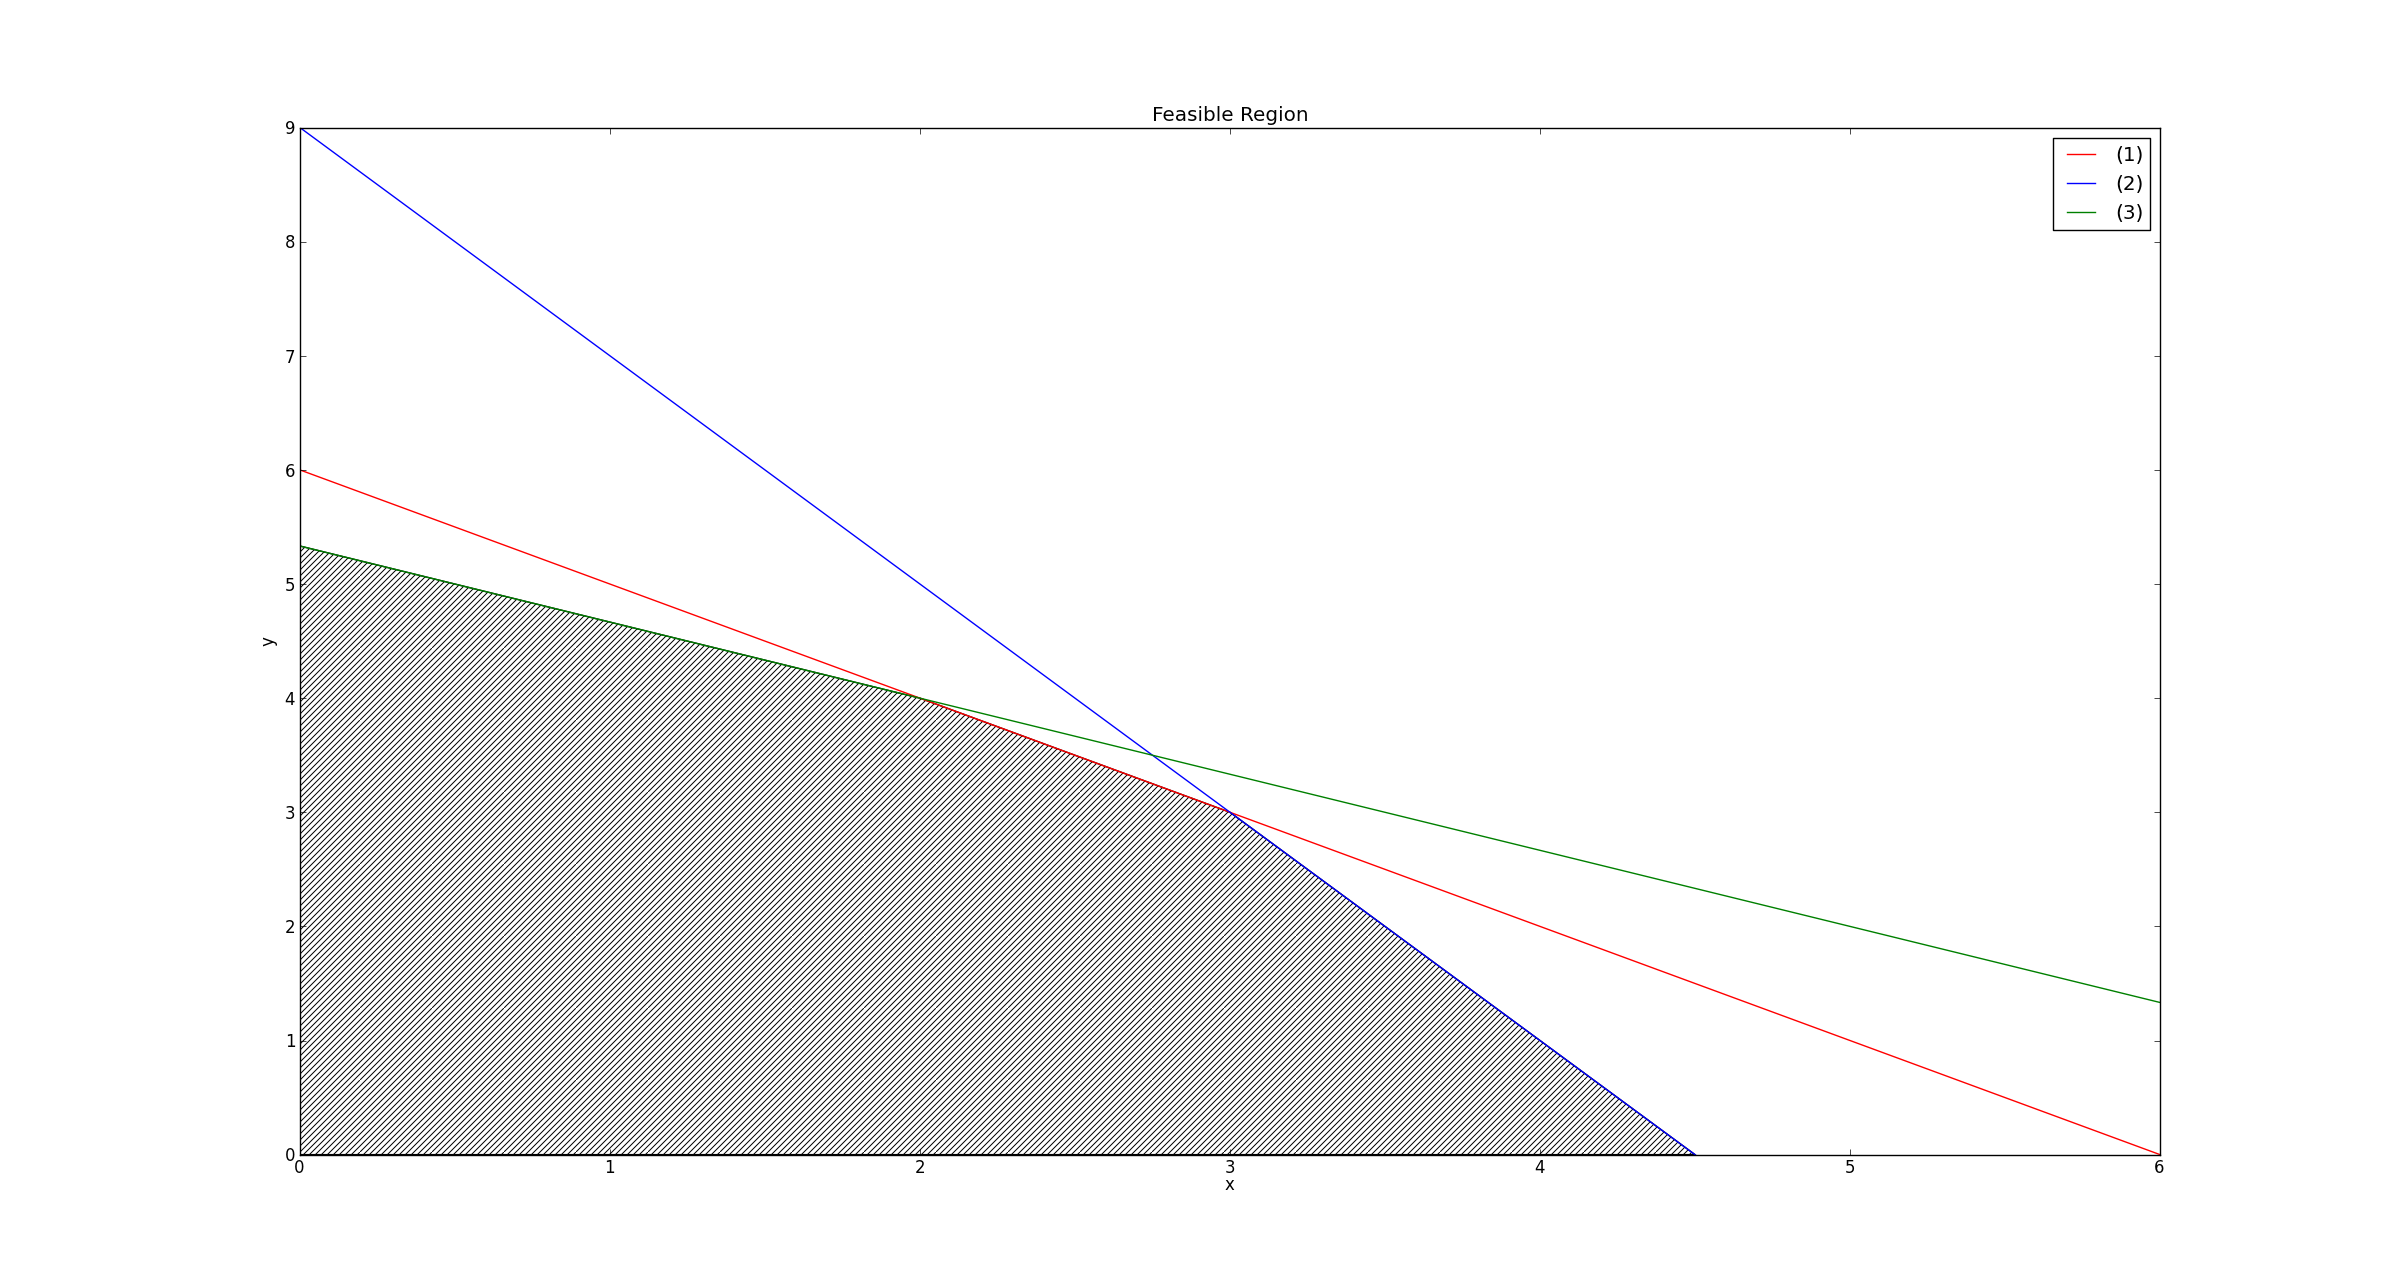
\includegraphics[scale=0.2]{feasible_region.png}
\end{frame}

\begin{frame}
\frametitle{Linear Programming Geometry}
\tiny
\begin{itemize}
\item Plot the objective function $z = 6x + 4y$ for some fixed values of $z$.
\item These are the so-called {\em isoprofit lines} or {\em objective function contours}.
\item Increasing $z$ results in a parallel shift to the right.
\end{itemize}
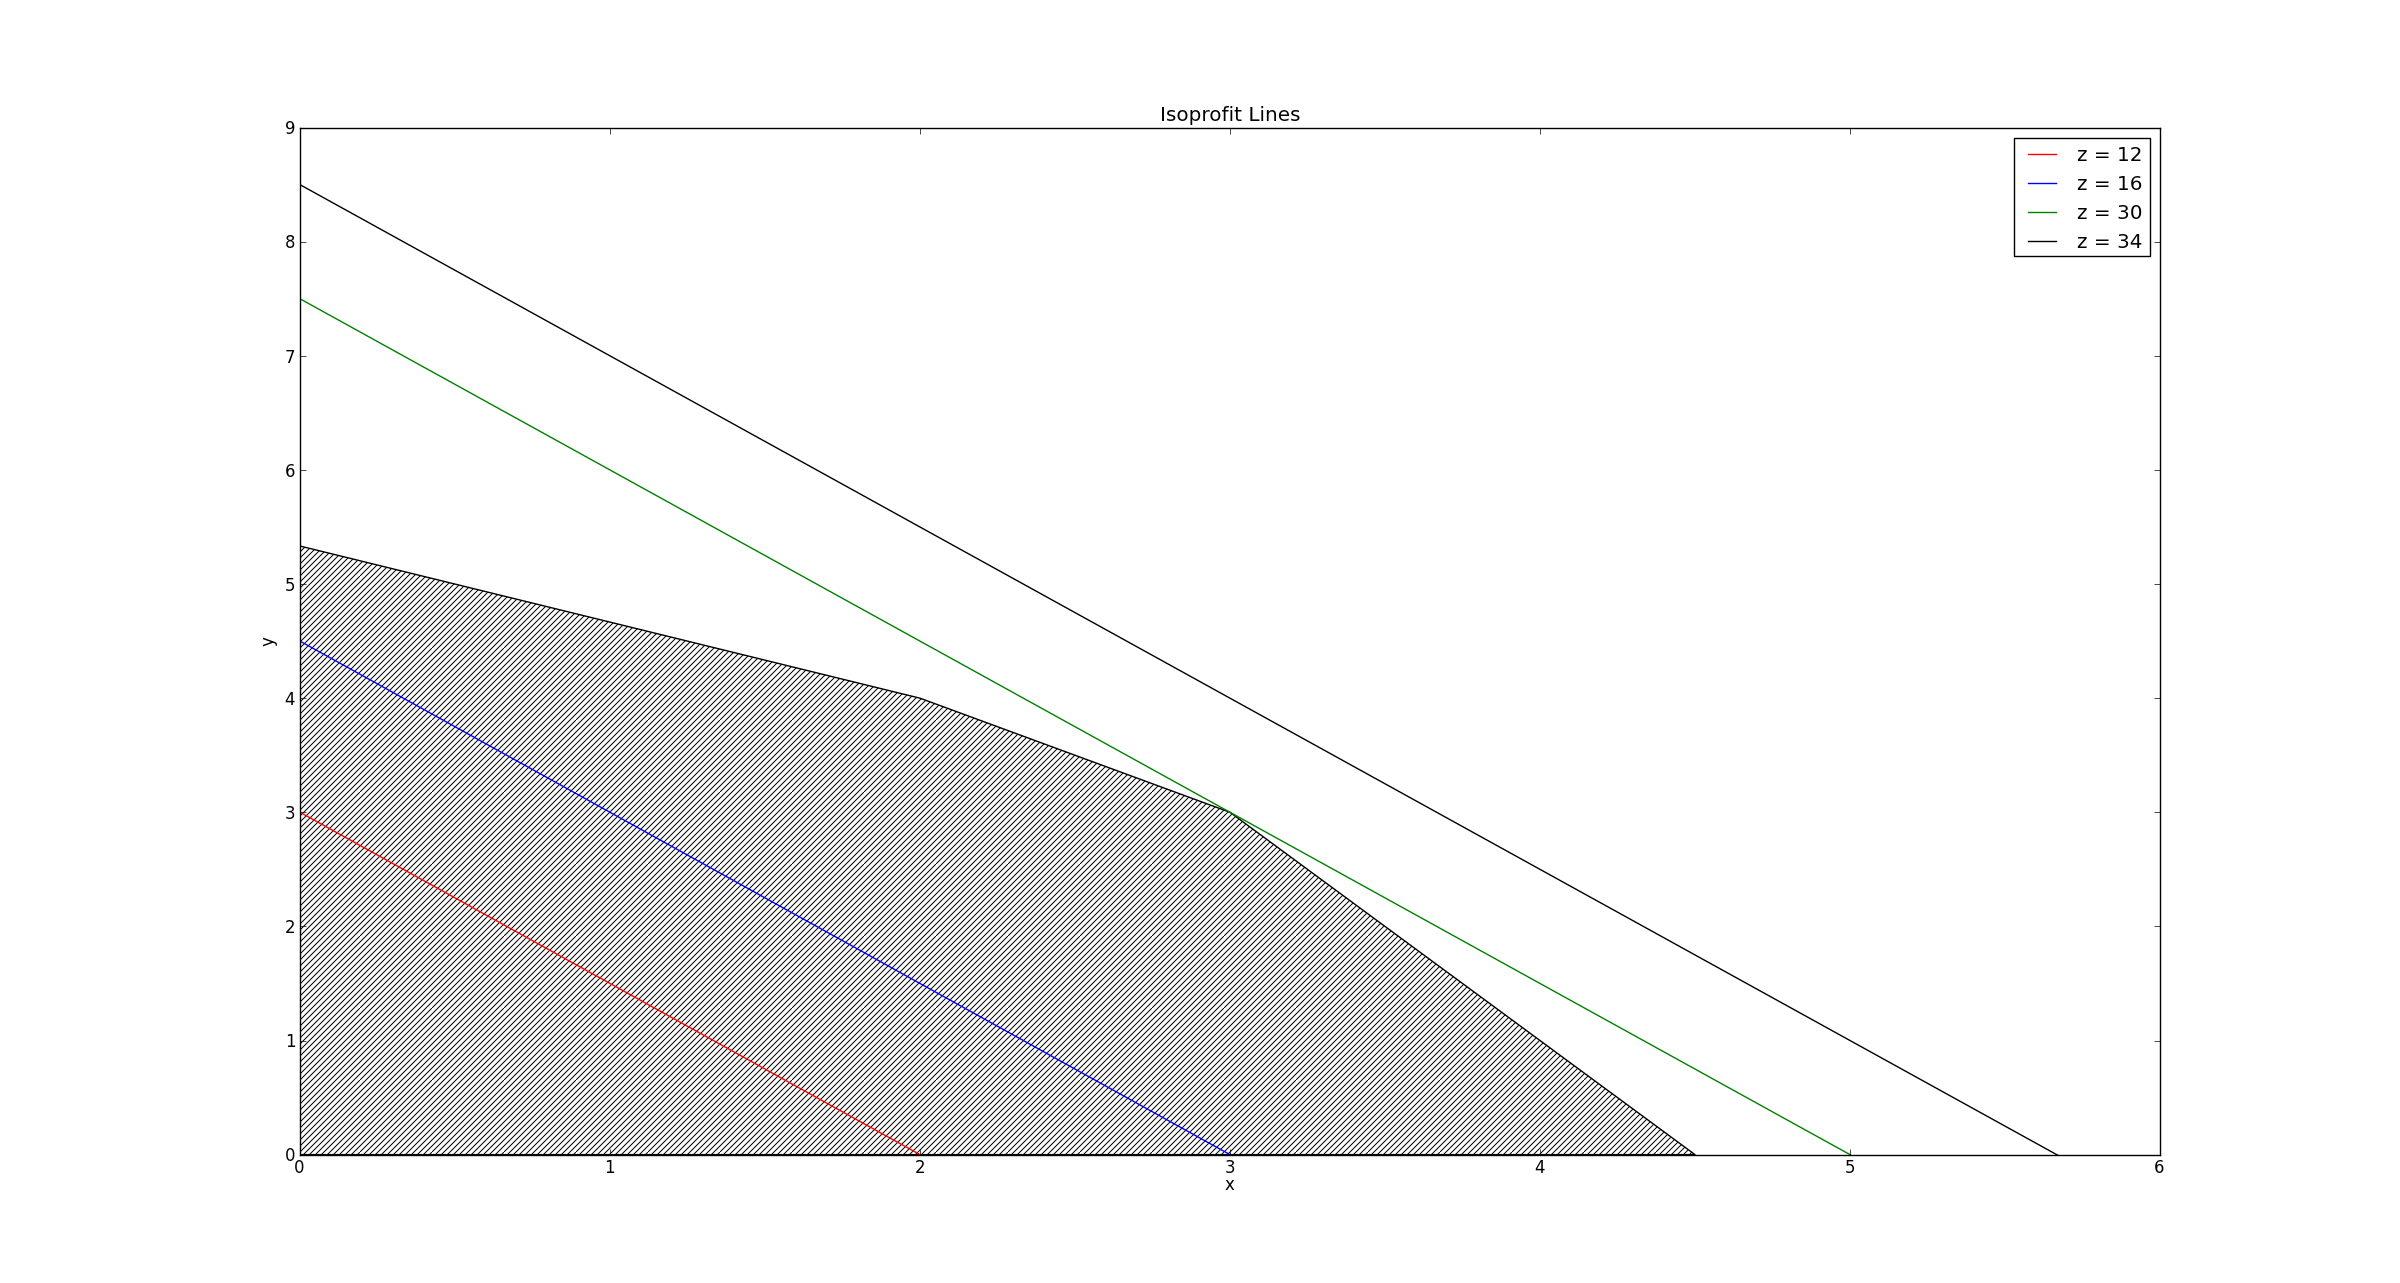
\includegraphics[scale=0.2]{isoprofit_lines.png}
\end{frame}

\begin{frame}
\frametitle{Observations}
\begin{itemize}
\item Feasible region of a linear program is always a convex polyhedron
\item At least one optimal solution occurs at a corner point (a.k.a. extreme point or vertex) of this polyhedron
\item Infinitely-many points in the feasible region, but only finitely many corner points
\end{itemize}
\end{frame}

\begin{frame}
\frametitle{Linear Programming Algebra}
First, how to solve linear systems of equations?
\begin{eqnarray}
2 x_1 + 1 x_2 + 1 x_3 &=& 4 \nonumber \\
4 x_1 - 6 x_2 + 0 x_3 &=& 2 \nonumber \\
-2 x_1 + 7 x_2 + 2 x_3 &=& 1 \nonumber
\end{eqnarray}
Systematically perform row operations to form equivalent systems
\begin{center}
Row 1 $\leftarrow \frac{1}{2}$ Row 1 \\
Row 2 $\leftarrow$ Row 2 - 4 Row 1 \\
Row 3 $\leftarrow$ Row 3 + 2 Row 1 \\
$\vdots$ \\
\end{center}
Until we arrive at an equivalent system with an obvious solution
\begin{eqnarray}
1 x_1 + 0 x_2 + 0 x_3 &=& 2 \nonumber \\
0 x_1 + 1 x_2 + 0 x_3 &=& 1 \nonumber \\
0 x_1 + 0 x_2 + 1 x_3 &=& 1 \nonumber
\end{eqnarray}
\end{frame}

\begin{frame}
\frametitle{Linear Programming Algebra}
\tiny
\begin{eqnarray}
\max_{x,y} && 6x + 4y = z \nonumber \\
\mbox{s.t.} && x + y \le 6 \nonumber \\
&& 2x + y \le 9 \nonumber \\
&& 2x + 3y \le 16 \nonumber \\
&& x, y \ge 0 \nonumber
\end{eqnarray}
As a system of linear equations:
\begin{eqnarray}
\max_{x,y,s} && 6x + 4y + 0 s_1 + 0 s_2 + 0 s_3 = z\nonumber \\
\mbox{s.t.} && 1x + 1y + 1s_1 + 0 s_2 + 0 s_3 = 6 \nonumber \\
&& 2x + 1y + 0s_1 + 1s_2 + 0s_3 = 9 \nonumber \\
&& 2x + 3y + 0s_1 + 0s_2 + 1s_3 = 16 \nonumber \\
&& x, y, s_1, s_2, s_3 \ge 0 \nonumber
\end{eqnarray}
Add the objective as the equation $-z + 6x + 4y = 0$ and write in matrix form:
\begin{eqnarray}
\left[ \begin{array}{rrrrrr|r}
z & x & y & s_1 & s_2 & s_3 & RHS \\
-1 & 6 & 4 & 0 & 0 & 0 & 0 \\
0 & 1 & 1 & 1 & 0 & 0 & 6 \\
0 & 2 & 1 & 0 & 1 & 0 & 9 \\
0 & 2 & 3 & 0 & 0 & 1 & 16
\end{array} \right] \nonumber
\end{eqnarray}
\end{frame}

\begin{frame}
\frametitle{Linear Programming Algebra}
\tiny
\begin{eqnarray}
\left[ \begin{array}{rrrrrr|r}
z & x & y & s_1 & s_2 & s_3 & RHS \\
-1 & 6 & 4 & 0 & 0 & 0 & 0 \\
0 & 1 & 1 & 1 & 0 & 0 & 6 \\
0 & 2 & 1 & 0 & 1 & 0 & 9 \\
0 & 2 & 3 & 0 & 0 & 1 & 16
\end{array} \right] \nonumber
\end{eqnarray}
Systematically perform row operations
\begin{eqnarray}
\left[ \begin{array}{rrrrrr|r}
z & x & y & s_1 & s_2 & s_3 & RHS \\
-1 & 0 & 1 & 0 & -3 & 0 & -27 \\
0 & 0 & 1/2 & 1 & -1/2 & 0 & 3/2 \\
0 & 1 & 1/2 & 0 & 1/2 & 0 & 9/2 \\
0 & 0 & 2 & 0 & -1 & 1 & 7
\end{array} \right] \nonumber
\end{eqnarray}
Until the solution is obvious
\begin{eqnarray}
\left[ \begin{array}{rrrrrr|r}
z & x & y & s_1 & s_2 & s_3 & RHS \\
-1 & 0 & 0 & -2 & -2 & 0 & -30 \\
0 & 0 & 1 & 2 & -1 & 0 & 3 \\
0 & 1 & 0 & -1 & 1 & 0 & 3 \\
0 & 0 & 0 & -4 & 1 & 1 & 1
\end{array} \right] \nonumber
\end{eqnarray}
What is the obvious solution? This is the equivalent LP:
\begin{eqnarray}
\max_{x, y, s} && 0 x + 0 y - 2 s_1 - 2 s_2 + 0 s_3 + 30 = z\nonumber \\
\mbox{s.t.} && 0x + 1y + 2 s_1 - 1s_2 + 0 s_3 = 3 \nonumber \\
&& 1x + 0y - 1s_1 + 1s_2 + 0 s_3 = 3 \nonumber \\
&& 0x + 0y - 4s_1 + 1s_2 + 1s_3 = 1 \nonumber \\
&& x,y,s_1,s_2,s_3 \ge 0 \nonumber
\end{eqnarray}
\vskip -0.05 in
The optimal solution to this transformed LP is $(x, y, s_1, s_2, s_3) = (3, 3, 0, 0, 1)$, $z^* = 30$
\end{frame}

\begin{frame}
\frametitle{Linear Programming Algebra}
\tiny
In more detail
\begin{eqnarray}
\left[ \begin{array}{rrrrrr|r}
z & x & y & s_1 & s_2 & s_3 & RHS \\
-1 & 6 & 4 & 0 & 0 & 0 & 0 \\
0 & 1 & 1 & 1 & 0 & 0 & 6 \\
0 & \color{red}2 & 1 & 0 & 1 & 0 & 9 \\
0 & 2 & 3 & 0 & 0 & 1 & 16
\end{array} \right] \nonumber
\end{eqnarray}
Feasible solution $(x, y, s_1, s_2, s_3) = (0, 0, 6, 9, 16)$, $z = 0$. Increase $x$ since it has a positive coefficient.
\begin{eqnarray}
\left[ \begin{array}{rrrrrr|r}
z & x & y & s_1 & s_2 & s_3 & RHS \\
-1 & 0 & 1 & 0 & -3 & 0 & -27 \\
0 & 0 & \color{red}1/2 & 1 & -1/2 & 0 & 3/2 \\
0 & 1 & 1/2 & 0 & 1/2 & 0 & 9/2 \\
0 & 0 & 2 & 0 & -1 & 1 & 7
\end{array} \right] \nonumber
\end{eqnarray}
Feasible solution $(x, y, s_1, s_2, s_3) = (9/2, 0, 3/2, 0, 7)$, $z = 27$. Increase $y$ since it has a positive coefficient.
\begin{eqnarray}
\left[ \begin{array}{rrrrrr|r}
z & x & y & s_1 & s_2 & s_3 & RHS \\
-1 & 0 & 0 & -2 & -2 & 0 & -30 \\
0 & 0 & 1 & 2 & -1 & 0 & 3 \\
0 & 1 & 0 & -1 & 1 & 0 & 3 \\
0 & 0 & 0 & -4 & 1 & 1 & 1
\end{array} \right] \nonumber
\end{eqnarray}
Feasible solution $(x, y, s_1, s_2, s_3) = (3, 3, 0, 0, 1)$, $z = 30$. \\
Transformed objective has no positive coefficients. \\
Transformed constraints have an ``obvious'' solution in which all variables with a negative objective coefficient are zero. \\
This is a provably optimal solution.
\end{frame}
\begin{frame}
\frametitle{Observations}
\begin{itemize}
\item Each iteration maintained exactly 3 positive decision variables (one for each of the original structural constraints).
\item The set of positive variables is {\em basis} (and the associated solution is a {\em basic feasible solution}).
\item Each iteration adds a new variable to a basis, and kicks an old variable out.
\item The objective improves at each iteration.
\item Proof of optimality: transformed objective coefficients are zero for basic variables, non-positive for non-basic variables.
\item What would change if we perturbed the original
\begin{itemize}
\item objective function coefficients?
\item right-hand sides?
\end{itemize}
\end{itemize}
\end{frame}
\begin{frame}
\frametitle{Connecting the Algebra to the Geometry}
We iterated over basic feasible solutions $(0, 0, 6, 9, 16)$, $(9/2, 0, 3/2, 0, 7)$, and $(3, 3, 0, 0, 1)$. Plotting these points in $(x,y)$ space...
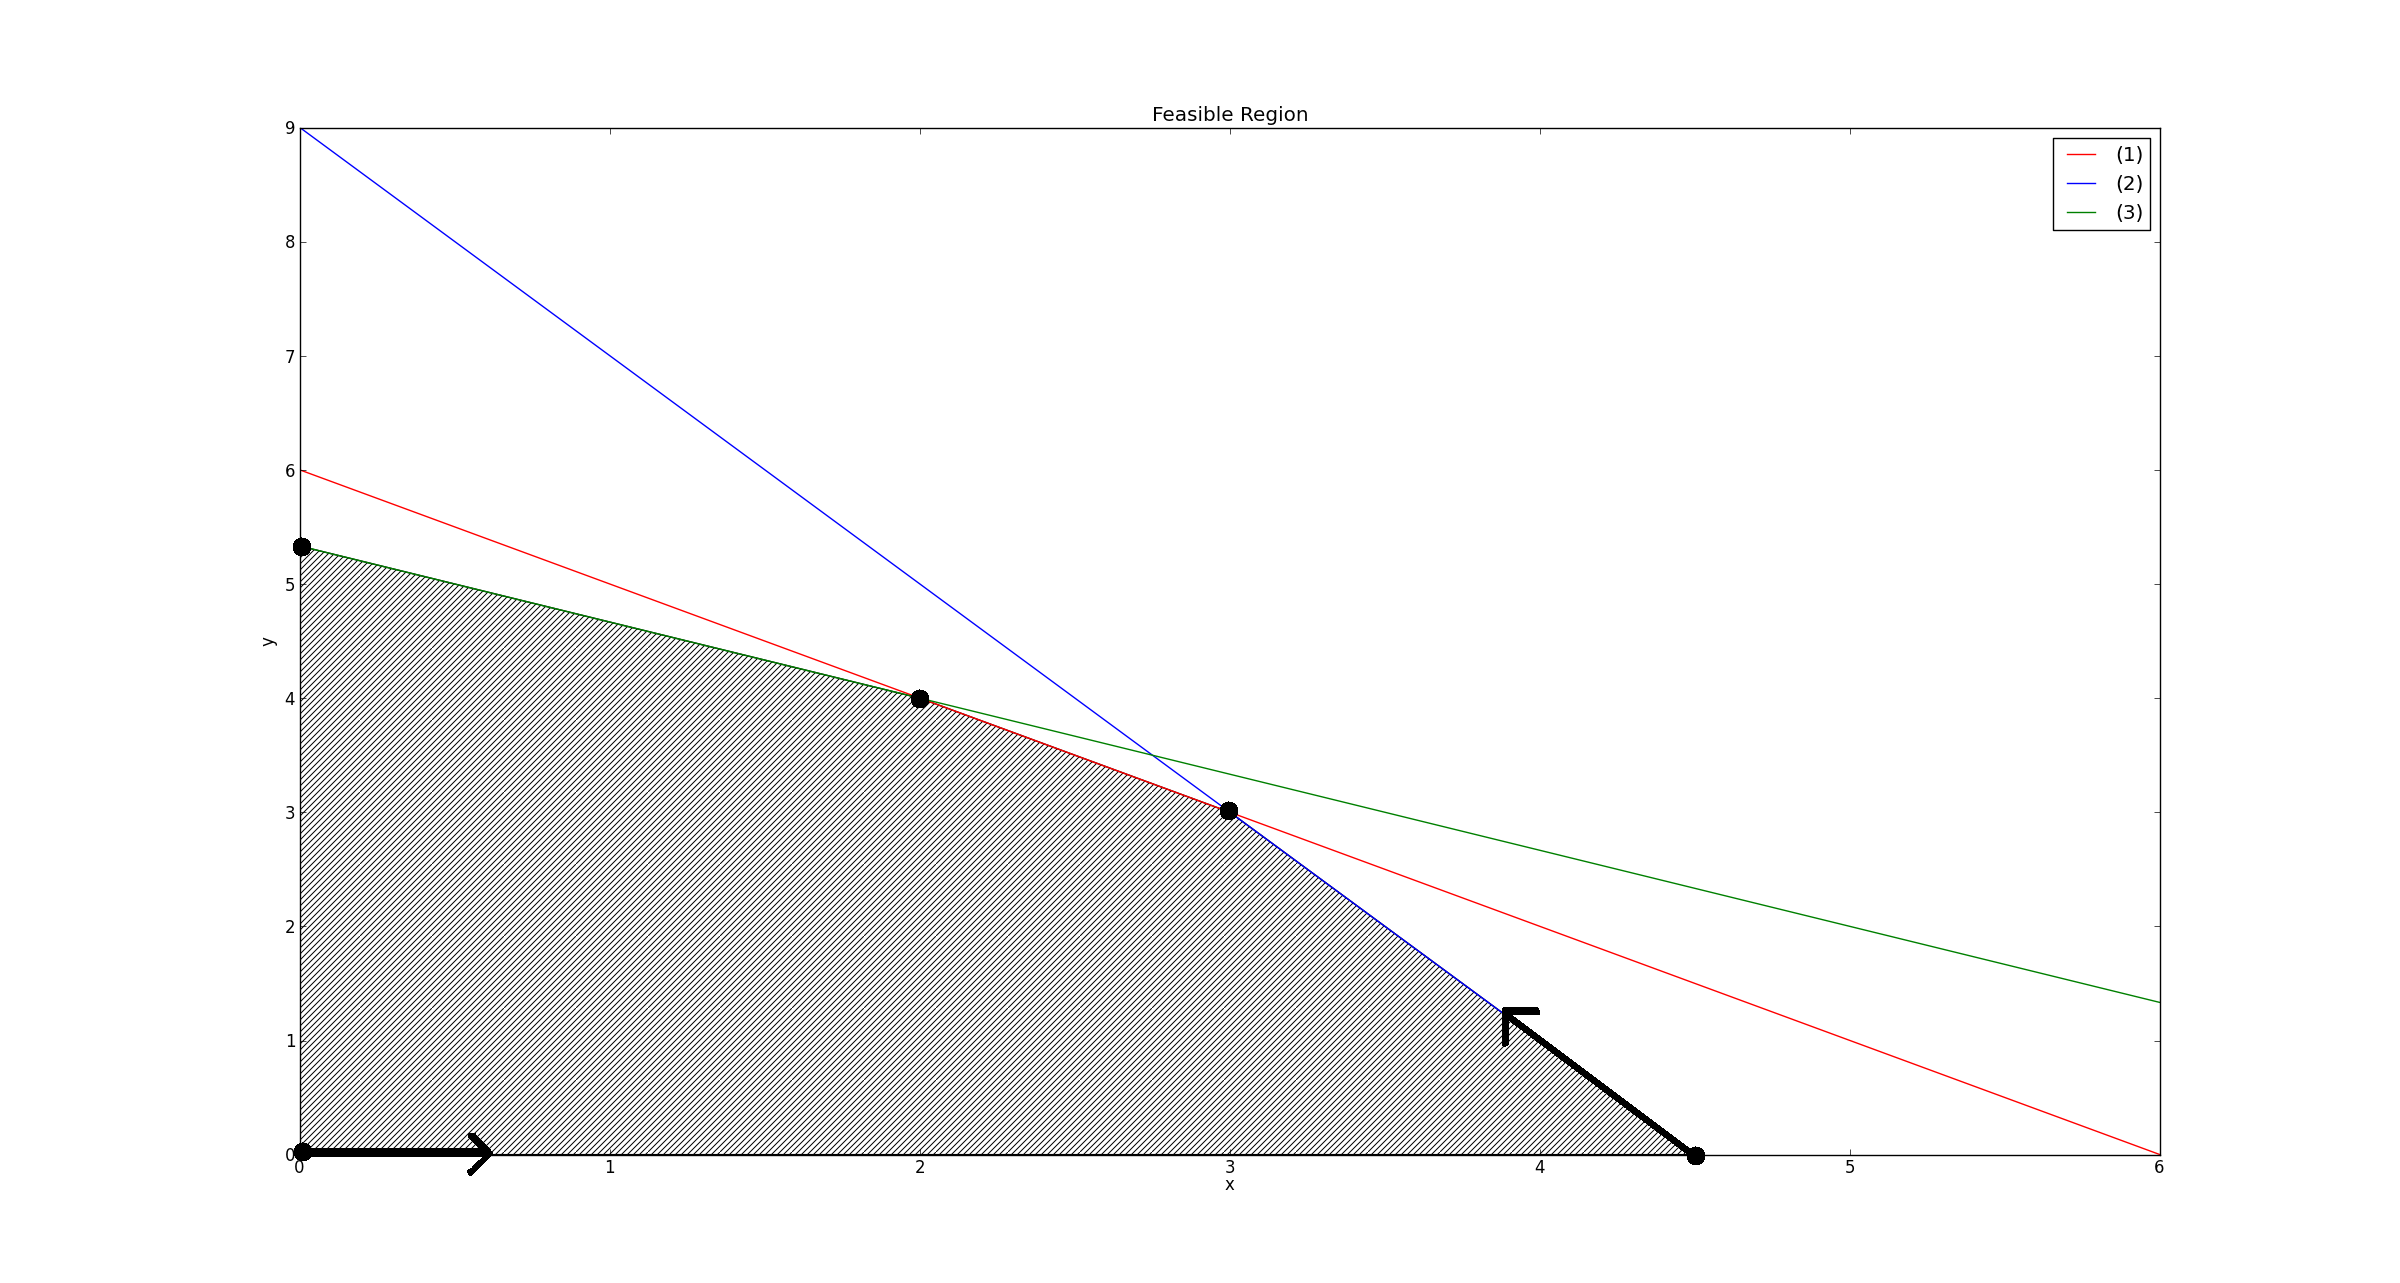
\includegraphics[scale=0.15]{simplex_iterations.png}
\end{frame}

\begin{frame}
\frametitle{Exercises}
\begin{itemize}
\item Solve the preceding model with Gurobi.
    \begin{itemize}
    \item Note: Set the model attribute ModelSense to -1 in order to maximize
    \end{itemize}
\item Which constraints are tight at the optimal solution?
\item Besides the origin, the feasible region has three other extreme points that are suboptimal under the current objective function. How might you change the objective function coefficients so that:
    \begin{itemize}
    \item the extreme point at $(0, \frac{16}{3})$ is optimal?
    \item the extreme point at $(\frac{9}{2}, 0)$ is optimal?
    \item all points between $(2, 4)$ and $(3, 3)$ are optimal?
    \end{itemize}
\end{itemize}
\end{frame}

\begin{frame}
\frametitle{Possible Outcomes of an LP}
\begin{itemize}
\item Infeasible - feasible region is empty, i.e., $x_1 \ge 0$, $x_1 \le -1$
\item Unbounded - no finite optimum, i.e. $\mbox{max}\;\; 15 x_1$ subject to $x_1 \ge 0$
\item Multiple optima, i.e. $\mbox{max}\;\; 3x_1 + 3x_2$ subject to $x_1 + x_2 \le 1$ and non-negative
\item Unique optimal solution (as in previous example)
\end{itemize}
\end{frame}

\begin{frame}
\frametitle{Linear Programming Solver}
\begin{itemize}
  \item Finds {\em \bf an} optimal solution if feasible region is non-empty and objective function is bounded
  \item Might be multiple optimal solutions
  \begin{itemize}
    \item Which optimal solution returned is not defined.
  \end{itemize}
  \item Constraints are ``hard''
  \begin{itemize}
    \item Won't violate constraints \footnote{by more than the numerical tolerance} even if it helps the objective.
    \item Will tell if relaxing a constraint would help the objective.
  \end{itemize}
\item Solver makes no apologies for this behavior!
\item Includes proof of optimality
\end{itemize}
\end{frame}

\frame{\frametitle{Real Linear Programming Solvers}
Strengths
\begin{itemize}
  \item Can Solve very large problems in Practice
    \begin{itemize}
      \item Tuned for real-world business problems
      \item Routinely solve problems with $10^7$ variables and constraints
      \item Multiple Algorithms (controlled by parameter Method)
    \end{itemize}
\end{itemize}
Weaknesses
\begin{itemize}
  \item Don't guarantee a time to a solution
  \item Might not reach optimality (but will tell you if it doesn't)
  \item Work with floating point values
  \begin{itemize}
    \item Might violate constraints by a small tolerance (controlled by parameter FeasibilityTol)
    \item Might return a solution that is within some numerical tolerance of optimal (controlled by parameter OptimalityTol)
  \end{itemize}
\end{itemize}
The better the linear programming solver,
the less of an issue you will have with these realities.
}

\begin{frame}
\frametitle{Duality}
The diet problem, revisited:
\begin{eqnarray}
\min_x && 20x_1 + 10x_2 + 31x_3 + 11x_4 + 12x_5 \nonumber \\
\mbox{s.t.} && 2x_1 + 0x_2 + 3x_3 + 1x_4 + 2x_5 \ge 21 \nonumber \\
&& 0x_1 + 1x_2 + 2x_3 + 2x_4 + 1x_5 \ge 12 \nonumber \\
&& x_j \ge 0,\;\;j=1,2,\ldots, 5 \nonumber
\end{eqnarray}
Suppose we have pills that contain a single unit of iron or calcium. How much would someone solving the diet problem be willing to pay for these pills?
\end{frame}

\begin{frame}
\frametitle{Duality}
\begin{itemize}
\item Let $\pi_i, \pi_c$ be the price to be charged for an iron, calcium pill.
\item We wish to maximize total revenue of $v = 21 \pi_i + 12 \pi_c$.
\item We must charge prices that are competitive with the prices of the five food types.
    \begin{itemize}
    \item Each ounce of food type 1 provides 2 units of iron at a cost of 20, so $2\pi_i \le 20$.
    \item For food type 2, $\pi_c \le 10$.
    \item For food type 3, $3\pi_i + 2\pi_c \le 31$.
    \item For food type 4, $\pi_i + 2\pi_c \le 11$.
    \item For food type 5, $2\pi_i + \pi_c \le 12$.
    \end{itemize}
\item We don't want to give away our pills, so $\pi_i, \pi_c \ge 0$.
\end{itemize}
\end{frame}

\begin{frame}
\frametitle{Duality}
\small
The diet problem:
\begin{eqnarray}
z^* = \min_x && 20x_1 + 10x_2 + 31x_3 + 11x_4 + 12x_5 \nonumber \\
\mbox{s.t.} && 2x_1 + 0x_2 + 3x_3 + 1x_4 + 2x_5 \ge 21 \nonumber \\
&& 0x_1 + 1x_2 + 2x_3 + 2x_4 + 1x_5 \ge 12 \nonumber \\
&& x_j \ge 0,\;\;j=1,2,\ldots, 5 \nonumber
\end{eqnarray}
The ``dual'' problem:
\begin{eqnarray}
v^* = \max_\pi && 21 \pi_i + 12 \pi_c \nonumber \\
\mbox{s.t.} && 2\pi_i + 0\pi_c \le 20 \nonumber \\
&& 0\pi_i + 1\pi_c \le 10 \nonumber \\
&& 3\pi_i + 2\pi_c \le 31 \nonumber \\
&& 1\pi_i + 2\pi_c \le 11 \nonumber \\
&& 2\pi_i + 1\pi_c \le 12 \nonumber \\
&& \pi_i, \pi_c \ge 0 \nonumber
\end{eqnarray}
\end{frame}

\begin{frame}
\frametitle{Exercises}
\begin{itemize}
\item Intuitively, is it possible for $v^* > z^*$?
\item Solve the dual of the diet problem with Gurobi. (Maintain a copy of the Model object for the original diet problem for comparison purposes.)
\item How are $z^*$ and $v^*$ related?
\item How are $\pi_i^*$ and $\pi_c^*$ related to solution of the original diet problem?
\item Multiply the iron constraint in the original diet problem by $\pi_i^*$, the calcium constraint by $\pi_c^*$, and add the results.
    \begin{itemize}
    \item What is the resulting inequality?
    \item How can this inequality be used to prove optimality?
    \end{itemize}
\end{itemize}
\end{frame}

\begin{frame}
\frametitle{Computing Shadow Prices}
Gurobi computes $\pi$ for us even when we solve the primal. Recall that in the optimal solution to the diet problem example, only $x_4$ and $x_5$ were non-zero. Letting $b_i$ and $b_c$ be nutrient requirements, we have
\begin{eqnarray}
x_4 + 2 x_5 &=& b_i \nonumber \\
2 x_4 + x_5 &=& b_c \nonumber
\end{eqnarray}
We can solve for $x_4$ and $x_5$ as
\begin{eqnarray}
x_4 &=& -1/3 b_i + 2/3 b_c \nonumber \\
x_5 &=& 2/3 b_i - 1/3 b_c \nonumber
\end{eqnarray}
Plugging into the objective, we get
\begin{eqnarray}
z &=& 11x_4 + 12 x_5 \nonumber \\
&=& 11(-1/3 b_i + 2/3 b_c) + 12(2/3 b_i - 1/3 b_c) \nonumber \\
&=& 13/3 b_i + 10/3 b_c \nonumber
\end{eqnarray}
So, $\pi_i = 13/3$ and $\pi_c = 10/3$.
\end{frame}

\begin{frame}
\frametitle{Computing Reduced Costs}
\begin{itemize}
\item How are the reduced costs related to the shadow prices?
\item Consider food 3, which costs 31 per ounce and provides 3 units of iron and 2 units of calcium.
\item Iron is priced at 13/3 per unit, calcium at 10/3 per unit.
\item If we discount the cost of food 3 by the value of the nutrients that it provides, we get $31 - 3*(13/3) - 2*(10/3) = 34/3$, which is exactly the reduced cost.
\item What is the reduced cost for food 4?
\item How cheap would food type 3 need to be in order for it to be in our diet?
\item Suppose we introduce a new food that costs 20 per ounce and provides 2 units of iron and 3 units of calcium. Should we include this new food in our diet? Do we need to reoptimize?
\end{itemize}
\end{frame}

\begin{frame}
\frametitle{Notation}
Linear Programming involves exclusively addition and multiplication by constants.
The symbols $\in$ and $\notin$ is read as ``in'' and ``not in''.
If $I = \{1,2,3\}.$
\begin{block}{$$\sum_{i \in I} a_i x_i$$}
$$a_1 x_1 + a_2 x_2 + a_3 x_3$$
\end{block}
\begin{block}{$$x_i \le b_i \hspace{0.25in} \forall i \in I$$}
\begin{align*}
x_1 \le b_1 \\
x_2 \le b_2 \\
x_3 \le b_3 \\
\end{align*}
\end{block}
\end{frame}

\frame{\frametitle{Knapsack Problem}
\begin{itemize}
\item Set of items $I = \{1,\ldots,n\}$.
\item Each item has value $v_i$ and weight $w_i$.
\item Have a knapsack that with capacity $b$.
\item Can take part of any item.
\item What is the highest valued collection of items (and partial items) that can go into the knapsack?
\end{itemize}
\begin{eqnarray}
\max_x && \sum_{i \in I} v_i x_i \nonumber \\
\mbox{s.t.} && \sum_{i \in I} w_i x_i \le b \nonumber \\
&& 0 \le x_i \le 1,\;\;i \in I \nonumber
\end{eqnarray}
\begin{itemize}
\item Use a GRBLinExpr to build up the sum in the constraint.
\end{itemize}
}

\begin{frame} [containsverbatim]
\frametitle{.NET Implementation}
\tiny
\begin{verbatim}
int capacity = ...;int[] weights = ...;int[] profits = ...;
int nItems = weights.Length;

GRBVar[] itemSelected = new GRBVar[nItems];
GRBLinExpr totalKnapsackWeight = new GRBLinExpr();
for (int i = 0; i < nItems; ++i) {
    itemSelected[i] = m.AddVar(0, 1, profits[i], GRB.CONTINUOUS, "item_selected." + i);
    totalKnapsackWeight.AddTerm(weights[i], itemSelected[i]);
}
m.Update();
GRBConstr con = m.AddConstr(totalKnapsackWeight, 'L', capacity, "knapsack");
m.Set(GRB.IntAttr.ModelSense, GRB.MAXIMIZE);

m.Update();
m.Write("knapsack.lp");
m.Optimize();

if (m.get(GRB.IntAttr.Status) == GRB.OPTIMAL) {
    for (GRBVar var in m.GetVars()) {
        Console.WriteLine("{0} = {1}, reduced cost = {2}", var.Get(GRB.StringAttr.VarName),
                          var.Get(GRB.DoubleAttr.X), var.Get(GRB.DoubleAttr.RC));
    }
    for (GRBConstr constr in m.GetConstrs()) {
        Console.WriteLine("{0}, slack = {1}, pi = {2}", constr.get(GRB.StringAttr.ConstrName),
                          constr.get(GRB.DoubleAttr.Slack), constr.get(GRB.DoubleAttr.Pi));
    }
}
\end{verbatim}
\end{frame}

\frame{\frametitle{The Diet Problem Generalized}
\begin{itemize}
\item Sets and Indices
    \begin{itemize}
    \item $i \in I$: nutrients
    \item $j \in J$: food types
    \end{itemize}
\item Data
    \begin{itemize}
    \item $c_j$: per ounce cost food type $j$
    \item $a_{ij}$: quantity of nutrient $i$ per ounce of food type $j$
    \item $l_i$, $u_i$: min, max daily requirements for nutrient $i$
    \end{itemize}
\item Decision Variables
    \begin{itemize}
    \item $x_j$: the number of ounces to consume of
 food type $j$.
    \end{itemize}
\item Formulation?
\item Let $\pi_i$ be the shadow price for nutrient $i$. What is the reduced cost of food type $j$, in terms of $\pi$?
\end{itemize}
}

\begin{frame} [containsverbatim]
\frametitle{.NET Implementation}
Add ranged constraints to GRBModel via GRBModel.addRange(expr, lower, upper, name) \\
For example, $l_j \le \sum_{i \in I} a_{ij} x_i \le u_j,\;\;j \in J$ can be created via: \\
\small
\begin{verbatim}
for (int j = 0; j < J; ++j) {
    GRBLinExpr nutrientConsumption = new GRBLinExpr();
    for (int i = 0; i < I; ++i)
        nutrientConsumption.AddTerm(a[i][j], x[i]);
    model.AddRange(nutrientConsumption, l[j], u[j],
                   "nutrient_consumption." + j);
}
\end{verbatim}
\end{frame}

\begin{frame}
\frametitle{Transportation Problem}
\begin{center}
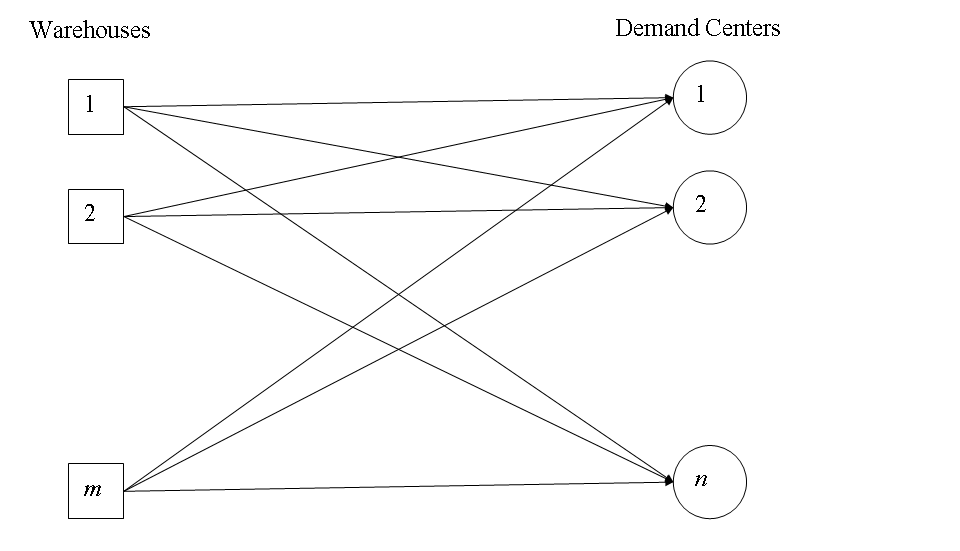
\includegraphics[scale = 0.3]{transportation_problem.png}
\end{center}
Input: \\
Warehouse capacity $u_i$ (widgets) \\
Customer demand $d_j$ (widgets) \\
Shipping cost $c_{ij}$ (\$/widget)
\end{frame}

\begin{frame}
\frametitle{Transportation Problem}
\begin{itemize}
\item Sets and Indices
    \begin{itemize}
    \item $i \in I$: Warehouses
    \item $j \in J$: Customers
    \end{itemize}
\item Data
    \begin{itemize}
    \item $u_i$: capacity for warehouse $i$ (widgets)
    \item $d_j$: demand at Customers $j$ (widgets)
    \item $c_{ij}$: shipping cost from warehouse $i$ to customer $j$ (\$/widget)
    \end{itemize}
\item Decision Variables
    \begin{itemize}
    \item $x_{ij}$: number of widgets to ship from warehouse $i$ to customer $j$
    \end{itemize}
\end{itemize}
\end{frame}

\begin{frame}
\frametitle{LP Formulation}
\begin{eqnarray}
\min_{x} && \sum_{i \in I} \sum_{j \in J} c_{ij} x_{ij} \;\; \mbox{(minimize shipping costs)} \nonumber \\
\mbox{s.t.} && \sum_{i \in I} x_{ij} = d_j,\;\;j \in J \;\; \mbox{(satisfy demand)}\nonumber \\
&& \sum_{j \in J} x_{ij} \le u_i,\;\;i \in I \;\; \mbox{(don't exceed capacity)} \nonumber \\
&& x_{ij} \ge 0, \;\;i \in I,\;j \in J \;\; \mbox{(ship nonnegative quantities)} \nonumber
\end{eqnarray}
\end{frame}

\begin{frame} [containsverbatim]
\frametitle{.NET Implementation}
Use GRBLinExpr to build up the summations in the constraints. \\
Assume $x$ is a 2d array of GRBVar and has already been populated. \\
Demand constraints $\sum_{i \in I} x_{ij} = d_j,\;\;j \in J$ are built via: \\
{\scriptsize
\begin{verbatim}
for (int j = 0; j < J; ++j) {
    GRBLinExpr unitsShippedToJ = new GRBLinExpr();
    for (int i = 0; i < I; ++i)
        unitsShippedToJ.AddTerm(1.0, x[i][j]);
    model.AddConstr(unitsShippedToJ, GRB.EQUAL, Demand[j], "Demand." + j);
}
\end{verbatim}
}

Capacity constraints $\sum_{j \in J} x_{ij} \le u_i,\;\;i \in I$ are built via: \\
{\scriptsize
\begin{verbatim}
for (int i = 0; i < I; ++i) {
  GRBLinExpr unitsShippedFromI = new GRBLinExpr();
  for (int j = 0; j < J; ++j)
    unitsShippedFromI.AddTerm(1.0, x[i][j]);
  model.AddConstr(unitsShippedFromI, GRB.LESS_EQUAL, Capacity[i], "Capacity." + i);
}
\end{verbatim}
\end{frame}
}
\begin{frame}
\frametitle{Diagnosing Infeasibility}
\begin{itemize}
\item After optimization, always check the Model attribute Status to determine whether the model was solved to optimality.
\item If Status is GRB.Status.Infeasible, how to diagnose infeasiblity?
\item GRBModel.computeIIS() computes an irreducible inconsistent subsystem.
\item Pass GRBModel.write() a filename with suffix .ilp to write the IIS to a file.
\item GRBVar attributes IISLB, IISUB indicate which variable bounds participate in the IIS.
\item GRBConstr attributes IISConstr indicate which constraints participate in the IIS.
\end{itemize}
\end{frame}

\begin{frame}
\frametitle{Exercise}
\begin{itemize}
\item Implement the transportation model with Gurobi.
\item Under what conditions would the problem become infeasible?
\item Create an infeasible instance, compute an IIS, and write it to a file.
\end{itemize}
\end{frame}

\begin{frame}
\frametitle{Softening Constraints}
To extend the transportation problem allow demand to go unsatisfied at a per-unit penalty of $\rho$ replace the demand constraint with
\begin{equation}
\sum_{i \in I} x_{ij} = d_j - y_j,\;\;j \in J, \nonumber
\end{equation}
\noindent where $y_j \ge 0$, and add $\rho \sum_{j \in J} y_j$ to the objective.
\end{frame}

\begin{frame}
\frametitle{Piecewise Linear Penalties}
Penalize the first 20\% of demand shortfall at a rate $\rho$, and any additional demand shortfall at a rate $1.5\rho$.
\begin{eqnarray}
\sum_{i \in I} x_{ij} = d_j - y_j^1 - y_j^2,\;\;j \in J \nonumber \\
0 \le y_j^1 \le 0.2d_j,\;\;j \in J \nonumber \\
0 \le y_j^2,\;\;j \in J, \nonumber
\end{eqnarray}
\noindent and add $\rho \sum_{j \in J} (y_j^1 + 1.5 y_j^2)$ to the objective.
\end{frame}


\begin{frame}
\frametitle{Minimize the Maximum Demand Shortfall}
\begin{itemize}
\item Recall: $\sum_{i \in I} x_{ij} = d_j - y_j,\;\;j \in J$
\item $y_j$ is the demand shortfall at demand center $j$.
\item Suppose we want to control $z = \max \{y_1, y_2, \ldots, y_n\}$.
\item Let $z \ge y_j,\;\;j \in J$.
\item Penalize $z$ in the objective, or put an upper bound on $z$.
\item Only works if we are trying to minimize $z$, otherwise we require integer variables.
\item Extends to any problem involving minimization (maximization) of the maximum (minimum) of several linear functions.
\item $y = |x|$ can be linearized as $y \ge x$, $y \ge -x$ (assuming minimization of $y$).
\end{itemize}
\end{frame}

\begin{frame}
\frametitle{Multiple Objectives}
\begin{eqnarray}
\min_{x} && \sum_{i \in I} \sum_{j \in J} c_{ij} x_{ij} + \rho \sum_{j \in J} y_j \nonumber \\
\mbox{s.t.} && \sum_{i \in I} x_{ij} = d_j - y_j,\;\;j \in J \nonumber \\
&& \sum_{j \in J} x_{ij} \le u_i,\;\;i \in I \nonumber \\
&& x_{ij} \ge 0, \;\;i \in I,\;j \in J \nonumber \\
&& y_j \ge 0,\;\;j \in J \nonumber
\end{eqnarray}
\begin{itemize}
\item Objectives:
    \begin{itemize}
    \item Minimize transportation cost $\sum_{i \in I} \sum_{j \in J} c_{ij} x_{ij}$
    \item Minimize demand shortfall $\sum_{j \in J} y_j$
    \end{itemize}
\item How do we choose $\rho$?
\end{itemize}
\end{frame}

\begin{frame}
\frametitle{Multiple Objectives}
\begin{itemize}
\item Generate an {\em efficient frontier} of solutions.
\item Let $z = \sum_{j \in J} y_j$.
\item Add $\rho z$ to the objective.
\item Optimize with $\rho = 0$.
\item Query GRBVar attribute SAObjUp.
\item Reoptimize with $\rho = (1+\epsilon)\mbox{SAObjUp}$.
\item LPs are cheap to reoptimize!
\end{itemize}
\end{frame}

\begin{frame}
\frametitle{Exercise}
Generate the efficient frontier of the transportation problem.
\end{frame}

\begin{frame} [containsverbatim]
\frametitle{Primary and Secondary Objectives}
\begin{itemize}
\item Optimize primary objective first.
\item Constrain primary objective to be within some tolerance of optimal.
\item Optimize secondary objective.
\end{itemize}
\small
\begin{verbatim}
GRBLinExpr primary = new GRBLinExpr();
GRBLinExpr secondary = new GRBLinExpr();
// build up objective functions
m.SetObjective(primary);
m.Optimize()
double objValue = model.Get(GRB.DoubleAttr.ObjVal);
m.AddConstr(primary, 'L', (1 + EPS)*objValue, "PrimaryObj");
m.SetObjective(secondary);
m.Optimize();
\end{verbatim}
\end{frame}

\frame{\frametitle{Shortest Path}
\begin{itemize}
\item Let $N$ be a set of cities.
\item Let $A$ be a set of arcs between cities.
\item Let $d_{ij}$ be the distance between city $i \in N$ and city $j \in N$.
\item What is the shortest distance between a given origin city $s \in N$ and destination city $t \in N$?
\end{itemize}
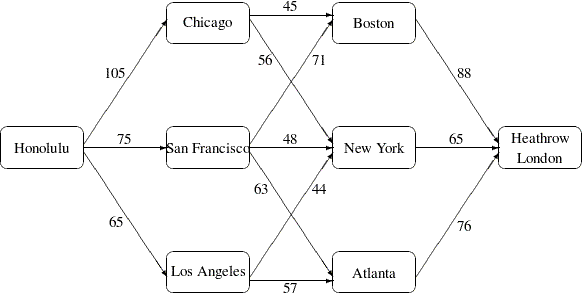
\includegraphics[scale=0.5]{netflow.png}
}

\begin{frame}
\frametitle{Shortest Path}
\begin{itemize}
\item Let $\pi_j$ be the length of the shortest path from the origin to city $j$.
\item Can write $\pi_j = \min_{(i,j) \in A} d_{ij} + \pi_i$ for every $j \in N$.
\item Linearize, and maximize $\pi_t$ to compute length of shortest path.
\item Tight constraints indicate arcs on the shortest path.
\end{itemize}
\begin{eqnarray}
\max_{\pi} && \pi_t \nonumber \\
\mbox{s.t.} && \pi_j \le \pi_i + d_{ij},\;\;(i,j) \in A \nonumber \\
&& \pi_s = 0 \nonumber
\end{eqnarray}
\end{frame}

\begin{frame}
\frametitle{Shortest Path}
Let $x_{ij} = 1$ if arc $(i,j)$ is traversed.
\begin{eqnarray}
\min_x && \sum_{(i,j) \in A} d_{ij} x_{ij} \nonumber \\
\mbox{s.t.} && \sum_{j \in FS(i)} x_{ij} - \sum_{j \in RS(i)} x_{ji} = b_i,\;\;i \in N \nonumber \\
&& 0 \le x_{ij} \le 1,\;\;(i,j) \in A, \nonumber
\end{eqnarray}
\noindent where $FS(i) = \{j | (i,j) \in A\}$, $RS(i) = \{j | (j, i) \in A\}$, $b_s = 1$, $b_t = -1$, and $b_i = 0$ for $i \neq s, t$.
\end{frame}

\begin{frame}
\frametitle{Exercise}
Implement both shortest path formulations. How are the two formulations related?
\end{frame}

\end{document}

